\documentclass{article}
\usepackage[T1]{fontenc}
\usepackage[utf8]{inputenc}
\usepackage[polish]{babel}
\usepackage{url}
\usepackage{amsmath}
\usepackage{amssymb}
\usepackage{graphicx}
\usepackage{booktabs}
\usepackage{float}
\usepackage{array}
\usepackage{multirow}
\usepackage{hyperref}
\graphicspath{{plots/}}
%{Informatyka stosowana 2022, I st., semestr VI}


\author{
    Mateusz Kosowski 251558 \\
    Nikodem Nowak 251598 \\
dr inż. Marcin Kacprowicz
}

\title{Komputerowe systemy rozpoznawania 2024/2025\\Projekt 2. Podsumowania lingwistyczne relacyjnych baz danych}
\begin{document}
\maketitle

Opis projektu ma formę artykułu naukowego lub raportu z zadania
badawczego (doświadczalnego/obliczeniowego (wg indywidualnych potrzeb związanych np. z
pracą inżynierską/naukową/zawodową). Wzory są numerowane, tablice są numerowane i podpisane nad
tablicą, rysunki są numerowane i podpisane pod rysunkiem. Podpis rysunku i
tabeli musi być wyczerpujący (nie ogólnikowy), aby czytelnik nie musiał sięgać do tekstu, aby go zrozumieć.\\
\indent {\bf Limit stron sprawozdania: 20. Nie zmieniać parametrów tekstu
(czcionki, marginesów, interlinii, itp.). Istotne dla sprawozdania rysunki,
tabele, informacje, kody itp. można umieścić w załącznikach, które nie wliczają
się do limitu stron.}\\
\indent {\bf Kolejne sekcje sprawozdania są uzupełniane wg wymagań w
opisie Projektu 2. i Harmonogramie Zajęć na WIKAMP KSR jako efekty zadań w~poszczególnych tygodniach}.

% =====================================================================
\section{Cel}

Celem projektu jest implementacja aplikacji desktopowej w technologii JDK
(Java 25 LTS) generującej \emph{lingwistyczne podsumowania} relacyjnej
bazy danych w formie zdań języka quasi-naturalnego. Aplikacja udostępnia
graficzny interfejs użytkownika, który dla użytkownika niezaawansowanego
pozwala wygenerować podsumowania na podstawie predefiniowanych
sumaryzatorów, kwalifikatorów i kwantyfikatorów (np. ,,samochody tanie
i stare''), zdefiniować wagi $w_i$ dla miar jakości,
posortować podsumowania według wybranej miary i zapisać wybrane wyniki
do pliku tekstowego, a~dla użytkownika zaawansowanego dodatkowo
zdefiniować nowe etykiety i funkcje przynależności.

Aplikacja generuje dwa rodzaje podsumowań:
\begin{itemize}
    \item \textbf{jednopodmiotowe} -- w pierwszej formie postaci ,,$Q$ obiektów
    ze zbioru ma własność $S$'' i drugiej formie postaci ,,$Q$ obiektów
    ze zbioru będących $W$ ma własność $S$'';
    \item \textbf{wielopodmiotowe} -- we wszystkich czterech formach
    (I.--IV.), porównujących dwa rozłączne podmioty $P_1, P_2$ ze zbioru
    (np. dwie różne marki samochodów),
\end{itemize}
gdzie $Q$ jest \emph{kwantyfikatorem lingwistycznym} (np. ,,większość'',
,,około połowy''), a $S$ i $W$ są \emph{sumaryzatorami} (kwalifikatorami)
zbudowanymi z etykiet zmiennych lingwistycznych powiązanych z atrybutami
bazy -- prostymi lub złożonymi za pomocą spójników logicznych. Dla każdego
wygenerowanego podsumowania aplikacja wyznacza miary jakości od~$T_1$
do~$T_{11}$ oraz miarę podsumowania optymalnego, na podstawie których
zwracane są uporządkowane rankingi podsumowań.

Aplikacja obsługuje trzy rodziny funkcji przynależności: trójkątną,
trapezoidalną i gaussowską. Dla wszystkich zmiennych lingwistycznych
i kwantyfikatorów w sprawozdaniu wybrano funkcje
\textbf{trapezoidalne} -- mają one prostą czteroparametrową definicję,
pozwalają w naturalny sposób uczynić skrajne etykiety lewo- i
prawo-otwartymi oraz łatwo zapewnić rozmyte pokrycie zupełne
uniwersum (sąsiednie etykiety nakładają się tak, że suma ich stopni
przynależności wynosi $1$).

Eksperymenty są prowadzone na podzbiorze $23\,441$ rekordów ze zbioru
\textit{Car Specification Dataset 1945--2020} (Kaggle, \cite{kaggle-cars}),
gromadzącego dane techniczne wersji wyposażenia samochodów osobowych
z~lat 1945--2020. Z oryginalnej bazy wybrano 12~atrybutów numerycznych
(rozmywanych do zmiennych lingwistycznych) oraz 3~atrybuty nominalne
(klucz, marka, model). Po odfiltrowaniu rekordów z brakującymi wartościami
otrzymano spójny zbiór wszystkich rekordów tego samego typu, do którego
zastosowanie narzędzi logiki rozmytej daje konkretne, zrozumiałe wnioski
o całej populacji aut.

Spodziewanym efektem jest zbiór rankingów podsumowań posortowanych według
miar jakości oraz wskazanie, które z miar $T_1$--$T_{11}$ niosą największą
informację o~badanej populacji aut, a~także które kombinacje
sumaryzatorów i kwantyfikatorów dają wartościowe (a które trywialne lub
mylące) opisy zawartości bazy.


% =====================================================================
\section{Baza danych, zmienne lingwistyczne, kwantyfikatory lingwistyczne}

% --------------------------------------------------------------
\subsection{Charakterystyka podsumowywanej bazy danych}
\label{sec:db}

Wykorzystany zbiór \textit{Car Specification Dataset 1945--2020}
\cite{kaggle-cars} zawiera $70\,823$ rekordów wersji wyposażenia
samochodów osobowych ($\,$\textit{trim level}$\,$) z~$255$ marek,
wyprodukowanych w~latach 1945--2020, opisanych $78$ atrybutami;
zbiór jest dostępny publicznie w~serwisie Kaggle. Każdy
rekord opisuje pojedynczą wersję wyposażenia jednego modelu, charakteryzując
ją zestawem cech technicznych
(wymiary, masa, parametry silnika, osiągi, zużycie paliwa, geometria
podwozia). Tego rodzaju dane są w~motoryzacji rutynowo opisywane językiem
naturalnym -- klient czy dziennikarz motoryzacyjny mówi raczej o
,,mocnym silniku'', ,,dużym SUV-ie'' albo ,,paliwożernym aucie'' niż o
konkretnych wartościach liczbowych $312$~KM,~$5\,300$~mm czy~$11{,}3$~l/100~km.
Z~tego powodu zbiór dobrze nadaje się do podsumowywania metodami
logiki rozmytej -- pozwala automatycznie generować zdania, które są
intuicyjne dla człowieka, a~trudne do uzyskania zwykłymi
zapytaniami SQL.

\paragraph{Wybór atrybutów i filtracja.} Z $78$ oryginalnych kolumn wybrano
\textbf{12 atrybutów numerycznych} podlegających rozmywaniu (są to atrybuty
mierzalne, każdy z wieloma setkami unikalnych wartości) oraz \textbf{3
atrybuty nominalne} pełniące funkcję klucza i etykiet podmiotów
w~podsumowaniach wielopodmiotowych. Z bazy odrzucono rekordy, w~których
przynajmniej jedna z 15~wybranych kolumn miała wartość pustą. Wynikowy
zbiór roboczy liczy $\mathbf{23\,441}$ \textbf{rekordów tego samego typu}
(z~$88$ marek), co spełnia wymóg minimum $10\,000$ rekordów w~projekcie.
Pełną listę atrybutów wraz z jednostkami i empirycznymi zakresami
przedstawia tabela~\ref{tab:atrybuty}.

\begin{table}[H]
\centering
\caption{Lista 15 atrybutów wybranych ze zbioru \textit{Car Specification Dataset 1945--2020}
\cite{kaggle-cars}: 12 numerycznych podlegających rozmyciu (zmienne lingwistyczne) oraz 3
nominalne wykorzystywane jako klucz/podmiot. Kolumna ,,zakres''
podaje zaobserwowane minimum i maksimum w~roboczym podzbiorze
$23\,441$ rekordów.}
\label{tab:atrybuty}
\resizebox{\textwidth}{!}{%
\begin{tabular}{l l l r}
\toprule
Atrybut (kolumna CSV) & Opis & Jednostka & Zakres \\
\midrule
\multicolumn{4}{l}{\textit{Atrybuty nominalne (klucz/podmiot):}} \\
\texttt{id\_trim} & Identyfikator wersji wyposażenia & --- & --- \\
\texttt{Make}     & Marka pojazdu                    & --- & 88 marek \\
\texttt{Modle}    & Model pojazdu                    & --- & --- \\
\midrule
\multicolumn{4}{l}{\textit{Atrybuty numeryczne (zmienne lingwistyczne):}} \\
\texttt{length\_mm}             & Długość całkowita pojazdu      & mm        & 1\,826 -- 6\,165 \\
\texttt{wheelbase\_mm}          & Rozstaw osi                    & mm        & 1\,397 -- 3\,872 \\
\texttt{curb\_weight\_kg}       & Masa własna pojazdu            & kg        & 625 -- 3\,000 \\
\texttt{minimum\_trunk\_capacity\_l} & Pojemność bagażnika       & l         & 11 -- 4\,400 \\
\texttt{maximum\_torque\_n\_m}  & Maksymalny moment obrotowy     & Nm        & 44 -- 1\,017 \\
\texttt{capacity\_cm3}          & Pojemność skokowa silnika      & cm$^3$    & 599 -- 7\,443 \\
\texttt{engine\_hp}             & Moc silnika                    & KM        & 29 -- 710 \\
\texttt{turning\_circle\_m}     & Średnica zawracania            & m         & 5{,}9 -- 19{,}5 \\
\texttt{mixed\_fuel\_consumption\_per\_100\_km\_l} & Spalanie mieszane & l/100 km & 1{,}4 -- 36{,}5 \\
\texttt{fuel\_tank\_capacity\_l}& Pojemność zbiornika paliwa     & l         & 10 -- 159 \\
\texttt{acceleration\_0\_100\_km/h\_s} & Czas przyspieszenia 0--100~km/h & s & 2{,}7 -- 33{,}2 \\
\texttt{max\_speed\_km\_per\_h} & Prędkość maksymalna            & km/h      & 100 -- 348 \\
\bottomrule
\end{tabular}}
\end{table}

Aby spełnić wymóg projektu dotyczący dostępu przez DBMS, przefiltrowane
dane są ładowane do pliku bazy \textbf{SQLite} (\texttt{cars.db}) jako
pojedyncza tabela \texttt{cars} i odczytywane przez aplikację Javową
przez sterownik JDBC. SQLite to w pełni relacyjny, plikowy system
zarządzania bazą danych -- nie wymaga osobnego serwera, ale obsługuje
SQL i transakcje dokładnie tak jak duże silniki (PostgreSQL, MySQL).
Fragment zawartości tabeli po wczytaniu przedstawia
tabela~\ref{tab:fragment}.

\begin{table}[H]
\centering
\caption{Fragment podzbioru roboczego (5 z 23\,441 rekordów). Kolumny
zostały skrócone do najważniejszych atrybutów dla zachowania czytelności;
pełny zestaw 15 atrybutów -- tabela~\ref{tab:atrybuty}. Wartości
przepisane bez modyfikacji ze zbioru źródłowego.}
\label{tab:fragment}
\resizebox{\textwidth}{!}{%
\begin{tabular}{l l r r r r r r r}
\toprule
Make & Model & dł.~[mm] & masa~[kg] & poj.~[cm$^3$] & moc~[KM] & 0--100~[s] & $V_{\max}$~[km/h] & sp.~[l] \\
\midrule
BMW            & 320i      & 4\,624 & 1\,495 & 1\,998 & 184 & 7{,}3  & 235 & 5{,}9 \\
Volkswagen     & Golf VII  & 4\,255 & 1\,205 & 1\,395 & 122 & 9{,}1  & 203 & 4{,}9 \\
Ford           & Fiesta VI & 3\,950 & 1\,041 & 1\,242 &  82 & 13{,}3 & 168 & 5{,}1 \\
Mercedes-Benz  & S 500     & 5\,246 & 2\,065 & 4\,663 & 455 & 4{,}8  & 250 & 9{,}1 \\
Toyota         & Aygo II   & 3\,455 &   840  &   998 &  72 & 14{,}2 & 160 & 4{,}1 \\
\bottomrule
\end{tabular}}
\end{table}

% --------------------------------------------------------------
\subsection{Zmienne lingwistyczne (atrybuty/własności obiektów)}
\label{sec:zmienne}

Każdy z~12 atrybutów numerycznych potraktowano jako \textbf{zmienną
lingwistyczną}, czyli atrybut, którego wartości można opisywać słowami
z~języka naturalnego zamiast surowych liczb -- np. zamiast ,,300~KM''
mówimy ,,silnik dynamiczny''. Dla każdej zmiennej trzeba ustalić trzy
rzeczy:
\begin{itemize}
    \item \textbf{przestrzeń rozważań} $X$ -- zakres wartości liczbowych
    atrybutu wyrażony w jego naturalnej jednostce (np. dla mocy silnika
    $X = [0, 800]$~KM);
    \item \textbf{zestaw etykiet} -- słowa, którymi opisujemy wartości
    z $X$ (np. ,,anemiczny / słaby / przyzwoity / dynamiczny / wyczynowy'');
    \item \textbf{funkcję przynależności} $\mu(x) \in [0, 1]$ dla każdej
    etykiety -- mówi ona, w jakim stopniu konkretna wartość liczbowa
    $x$ pasuje do danej etykiety (1 = w pełni, 0 = w ogóle).
\end{itemize}

\paragraph{Konwencja etykiet.} Dla każdej z~12 zmiennych przyjęto
\textbf{pięcioelementowy} zbiór etykiet $\mathcal{T}$ uporządkowany
według rosnącej wartości atrybutu, lecz \emph{dobrany indywidualnie}
do zmiennej z naturalnego, polskiego słownictwa motoryzacyjnego --
pozwala to uniknąć monotonnego ,,bardzo mała / mała / średnia / duża /
bardzo duża'' i nadać każdej zmiennej własny, czytelny dla człowieka
charakter (np. masa: ,,piórkowy -- masywny''; moc:
,,anemiczny -- wyczynowy''; spalanie: ,,oszczędny -- rozrzutny'').
Pełną listę etykiet dla każdej zmiennej zawierają tabele
\ref{tab:mf-length}--\ref{tab:mf-vmax} w kolejnych podpunktach.
Pięcioelementowy zestaw daje wystarczająco bogatą semantykę dla
podsumowań kolejnych tygodni (zarówno jedno-, jak i wielopodmiotowych)
przy zachowaniu czytelności wykresów; ujednolicenie liczby etykiet we
wszystkich zmiennych ułatwia konstruowanie sumarytorów złożonych
i porównywanie miar jakości między zmiennymi.

\paragraph{Funkcje przynależności.} We wszystkich 12 zmiennych
lingwistycznych i~we wszystkich kwantyfikatorach (\S\ref{sec:quant})
używamy \textbf{funkcji trapezoidalnej} -- ma cztery parametry
$a \le b \le c \le d$ i postać:
\begin{equation}
\label{eq:trapez}
    \mu_{(a,b,c,d)}(x) =
    \begin{cases}
        0, & x \le a \;\text{lub}\; x \ge d,\\[2pt]
        \dfrac{x-a}{b-a}, & a < x < b,\\[6pt]
        1, & b \le x \le c,\\[2pt]
        \dfrac{d-x}{d-c}, & c < x < d.
    \end{cases}
\end{equation}
Pierwsza i ostatnia etykieta każdej zmiennej (np. ,,piórkowy'' i
,,masywny'' dla masy) są odpowiednio \emph{lewo-} i \emph{prawo-otwarte}:
dla pierwszej przyjęto $a=b=x_{\min}$, a~dla ostatniej $c=d=x_{\max}$ --
dzięki temu zakres jest w~całości pokryty (skrajne wartości należą do
odpowiednio pierwszej lub ostatniej etykiety w stopniu $1$).
Sąsiednie trapezy są tak dobrane, że się ze sobą nakładają -- dla
każdej wartości $x$ suma stopni przynależności do wszystkich pięciu
etykiet wynosi w~przybliżeniu $1$, a w~punkcie przejścia między
sąsiednimi etykietami obie mają stopień $0{,}5$ (przykład:
rys.~\ref{fig:mf-engine-hp}).

\paragraph{Dobór parametrów.} Wartości parametrów $(a,b,c,d)$ dla
każdej z~5 etykiet wszystkich 12 zmiennych zebranych w~tabelach
\ref{tab:mf-length}--\ref{tab:mf-vmax} dobraliśmy w~ten sam sposób:
tak, żeby pasowały zarówno do faktycznego rozkładu danych w~zbiorze
(kwantyle 5\,\%, 25\,\%, 50\,\%, 75\,\%, 95\,\%), jak i do
ogólnych zasad obowiązujących w~motoryzacji. W~podpisach tabel
informacja ta nie jest powtarzana.

W~kolejnych podpunktach dla każdej zmiennej podano: przestrzeń rozważań
$X$, tabelę parametrów $(a,b,c,d)$ wszystkich pięciu etykiet oraz wykres
funkcji przynależności (linią ciągłą) wraz z~obszarem wsparcia
(odpowiadający kolorystycznie wypełnione obszary). Dla zaoszczędzenia
miejsca opis każdej zmiennej zajmuje pojedynczą tabelę i pojedynczy
rysunek.

% ----------- 12 zmiennych ------------

\subsubsection{Długość pojazdu (\texttt{length\_mm}), $X = [1500, 6500]$ mm}
\begin{table}[H]
\centering
\caption{Parametry trapezowych funkcji przynależności dla zmiennej
lingwistycznej ,,długość pojazdu''.}
\label{tab:mf-length}
\begin{tabular}{l r r r r}
\toprule
Etykieta & $a$ & $b$ & $c$ & $d$ \\
\midrule
krótki            & 1\,500 & 1\,500 & 3\,500 & 3\,900 \\
kompaktowy        & 3\,500 & 3\,900 & 4\,200 & 4\,500 \\
standardowy       & 4\,200 & 4\,500 & 4\,700 & 4\,900 \\
długi             & 4\,700 & 4\,900 & 5\,100 & 5\,300 \\
wielkogabarytowy  & 5\,100 & 5\,300 & 6\,500 & 6\,500 \\
\bottomrule
\end{tabular}
\end{table}
\begin{figure}[H]
\centering
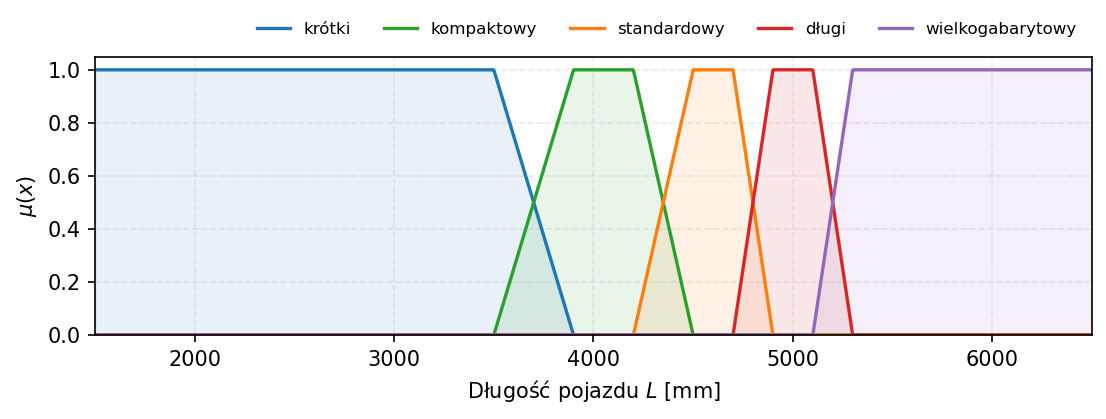
\includegraphics[width=0.9\textwidth]{mf_length_mm.png}
\caption{Funkcje przynależności pięciu etykiet zmiennej lingwistycznej
,,długość pojazdu'' $L \in [1500,6500]$~mm. Granice etykiet odpowiadają
segmentom Euro: A ($<$3,7 m), B (3,7--4,5 m), C/D (4,5--4,9 m),
E (4,9--5,3 m), F ($>$5,3 m).}
\label{fig:mf-length}
\end{figure}

\subsubsection{Rozstaw osi (\texttt{wheelbase\_mm}), $X = [1300, 4000]$ mm}
\begin{table}[H]
\centering
\caption{Parametry trapezowych funkcji przynależności dla zmiennej
,,rozstaw osi''.}
\label{tab:mf-wheelbase}
\begin{tabular}{l r r r r}
\toprule
Etykieta & $a$ & $b$ & $c$ & $d$ \\
\midrule
zwarty       & 1\,300 & 1\,300 & 2\,300 & 2\,450 \\
krótki       & 2\,300 & 2\,450 & 2\,550 & 2\,650 \\
standardowy  & 2\,550 & 2\,650 & 2\,750 & 2\,850 \\
wydłużony    & 2\,750 & 2\,850 & 2\,950 & 3\,050 \\
limuzynowy   & 2\,950 & 3\,050 & 4\,000 & 4\,000 \\
\bottomrule
\end{tabular}
\end{table}
\begin{figure}[H]
\centering
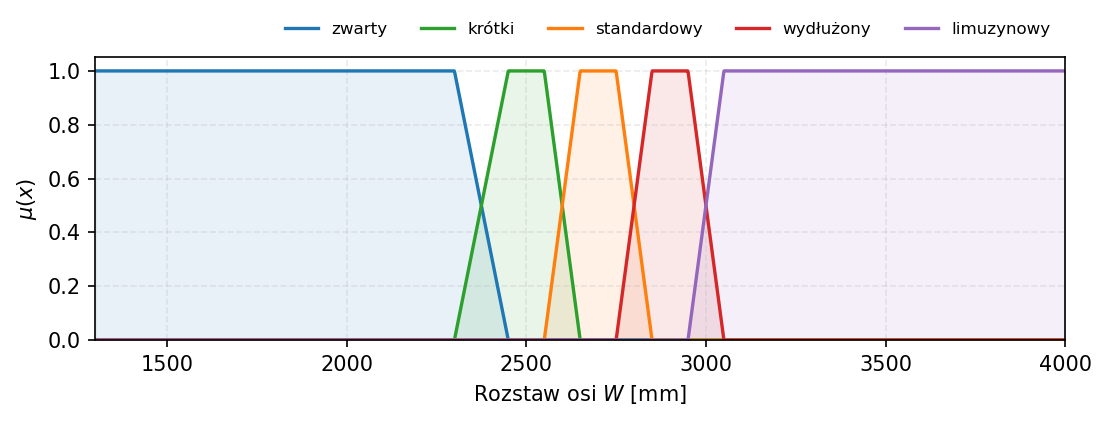
\includegraphics[width=0.9\textwidth]{mf_wheelbase_mm.png}
\caption{Funkcje przynależności pięciu etykiet zmiennej lingwistycznej
,,rozstaw osi'' $W \in [1300, 4000]$~mm.}
\label{fig:mf-wheelbase}
\end{figure}

\subsubsection{Masa własna (\texttt{curb\_weight\_kg}), $X = [500, 3500]$ kg}
\begin{table}[H]
\centering
\caption{Parametry trapezowych funkcji przynależności dla zmiennej
,,masa własna''.}
\label{tab:mf-mass}
\begin{tabular}{l r r r r}
\toprule
Etykieta & $a$ & $b$ & $c$ & $d$ \\
\midrule
piórkowy        &   500 &   500 &   900 & 1\,100 \\
lekki           &   900 & 1\,100 & 1\,250 & 1\,400 \\
średnio ciężki  & 1\,250 & 1\,400 & 1\,500 & 1\,650 \\
ciężki          & 1\,500 & 1\,650 & 1\,850 & 2\,050 \\
masywny         & 1\,850 & 2\,050 & 3\,500 & 3\,500 \\
\bottomrule
\end{tabular}
\end{table}
\begin{figure}[H]
\centering
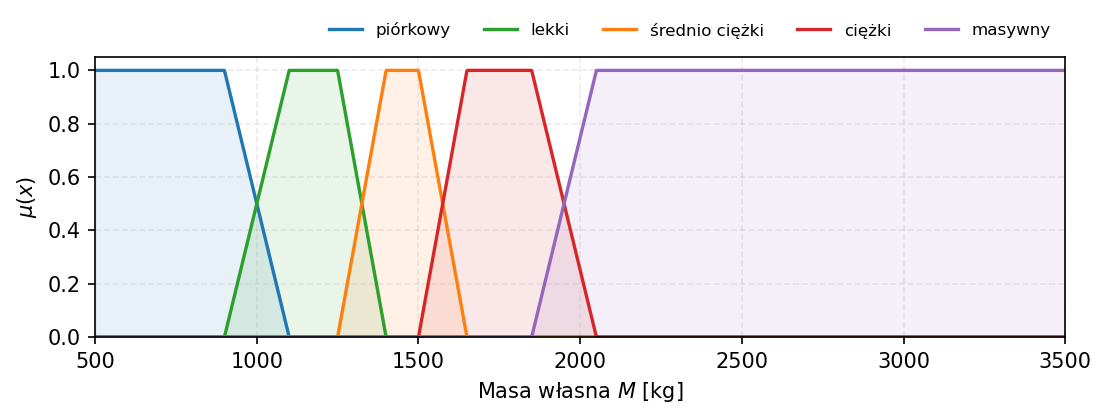
\includegraphics[width=0.9\textwidth]{mf_curb_weight_kg.png}
\caption{Funkcje przynależności pięciu etykiet zmiennej lingwistycznej
,,masa własna pojazdu'' $M \in [500, 3500]$~kg.}
\label{fig:mf-mass}
\end{figure}

\subsubsection{Pojemność bagażnika (\texttt{minimum\_trunk\_capacity\_l}), $X = [0, 1500]$ l}
\begin{table}[H]
\centering
\caption{Parametry trapezowych funkcji przynależności dla zmiennej
,,pojemność bagażnika''. Górna granica uniwersum ograniczona do
1500~l (rzadkie vany cargo z~$>$3000~l są wciąż poprawnie
sklasyfikowane jako ,,ładunkowy'').}
\label{tab:mf-trunk}
\begin{tabular}{l r r r r}
\toprule
Etykieta & $a$ & $b$ & $c$ & $d$ \\
\midrule
symboliczny   &   0 &   0 & 200 & 300 \\
ciasny        & 200 & 300 & 350 & 400 \\
standardowy   & 350 & 400 & 450 & 500 \\
pojemny       & 450 & 500 & 600 & 700 \\
ładunkowy     & 600 & 700 & 1\,500 & 1\,500 \\
\bottomrule
\end{tabular}
\end{table}
\begin{figure}[H]
\centering
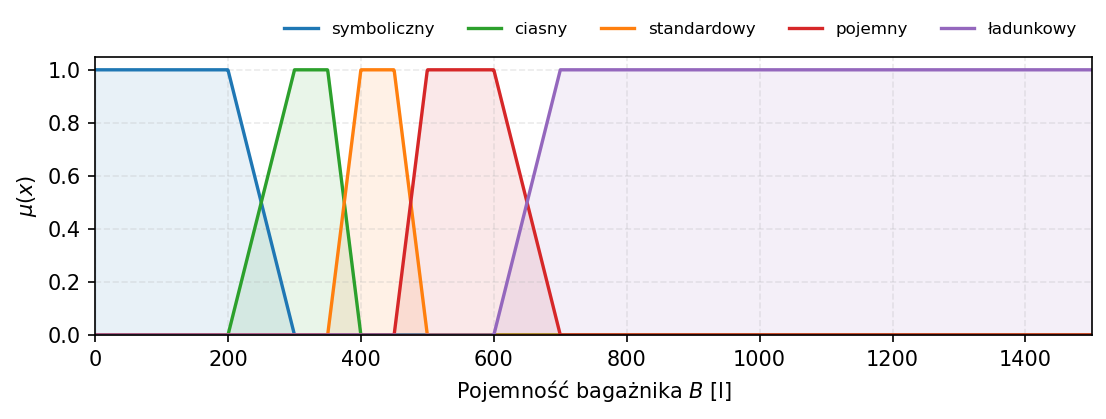
\includegraphics[width=0.9\textwidth]{mf_minimum_trunk_capacity_l.png}
\caption{Funkcje przynależności pięciu etykiet zmiennej lingwistycznej
,,pojemność bagażnika'' $B \in [0, 1500]$~l.}
\label{fig:mf-trunk}
\end{figure}

\subsubsection{Moment obrotowy (\texttt{maximum\_torque\_n\_m}), $X = [0, 1100]$ Nm}
\begin{table}[H]
\centering
\caption{Parametry trapezowych funkcji przynależności dla zmiennej
,,maksymalny moment obrotowy silnika''.}
\label{tab:mf-torque}
\begin{tabular}{l r r r r}
\toprule
Etykieta & $a$ & $b$ & $c$ & $d$ \\
\midrule
wiotki        &   0 &   0 & 100 & 150 \\
miękki        & 100 & 150 & 180 & 230 \\
zrównoważony  & 180 & 230 & 280 & 350 \\
mocarny       & 280 & 350 & 450 & 550 \\
potężny       & 450 & 550 & 1\,100 & 1\,100 \\
\bottomrule
\end{tabular}
\end{table}
\begin{figure}[H]
\centering
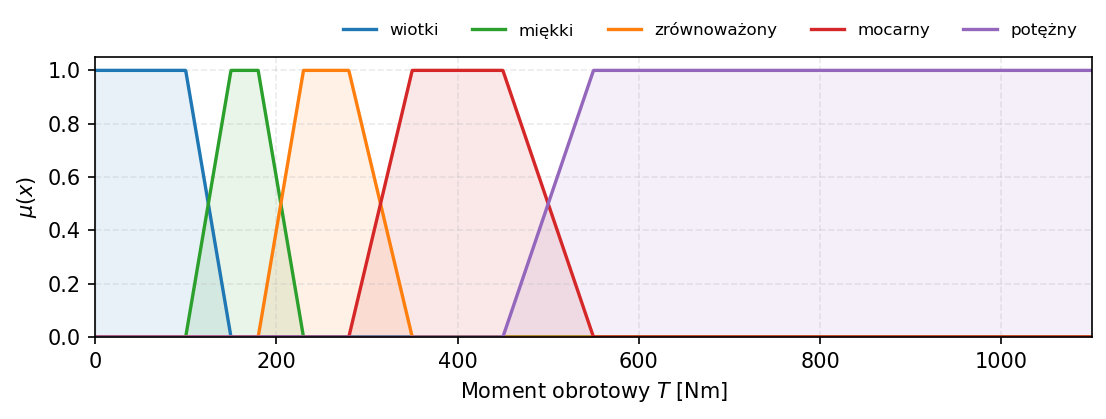
\includegraphics[width=0.9\textwidth]{mf_maximum_torque_n_m.png}
\caption{Funkcje przynależności pięciu etykiet zmiennej lingwistycznej
,,maksymalny moment obrotowy'' $T \in [0, 1100]$~Nm.}
\label{fig:mf-torque}
\end{figure}

\subsubsection{Pojemność skokowa silnika (\texttt{capacity\_cm3}), $X = [400, 8000]$ cm$^3$}
\begin{table}[H]
\centering
\caption{Parametry trapezowych funkcji przynależności dla zmiennej
,,pojemność skokowa''.}
\label{tab:mf-capacity}
\begin{tabular}{l r r r r}
\toprule
Etykieta & $a$ & $b$ & $c$ & $d$ \\
\midrule
miniaturowy        &   400 &   400 & 1\,200 & 1\,400 \\
małolitrażowy      & 1\,200 & 1\,400 & 1\,600 & 1\,800 \\
średniolitrażowy   & 1\,600 & 1\,800 & 2\,000 & 2\,500 \\
wielkolitrażowy    & 2\,000 & 2\,500 & 3\,500 & 4\,500 \\
gigantyczny        & 3\,500 & 4\,500 & 8\,000 & 8\,000 \\
\bottomrule
\end{tabular}
\end{table}
\begin{figure}[H]
\centering
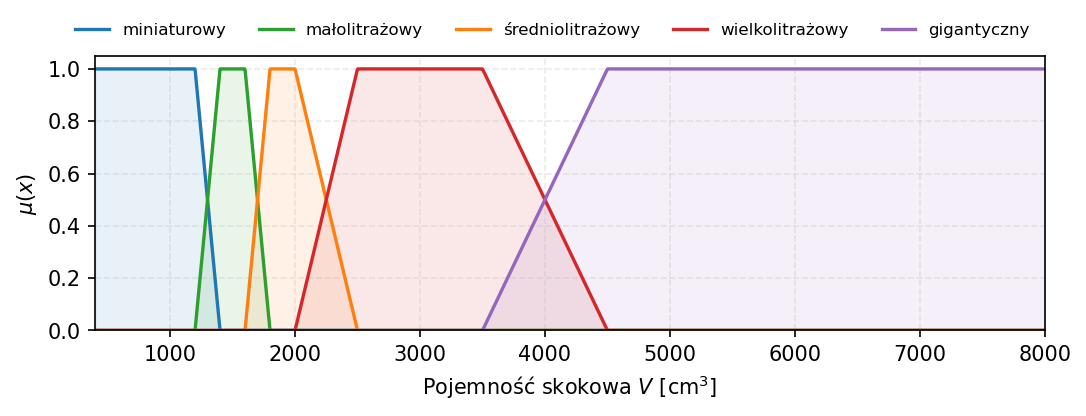
\includegraphics[width=0.9\textwidth]{mf_capacity_cm3.png}
\caption{Funkcje przynależności pięciu etykiet zmiennej lingwistycznej
,,pojemność skokowa silnika'' $V \in [400, 8000]$~cm$^3$.}
\label{fig:mf-capacity}
\end{figure}

\subsubsection{Moc silnika (\texttt{engine\_hp}), $X = [0, 800]$ KM}
\begin{table}[H]
\centering
\caption{Parametry trapezowych funkcji przynależności dla zmiennej
,,moc silnika''.}
\label{tab:mf-hp}
\begin{tabular}{l r r r r}
\toprule
Etykieta & $a$ & $b$ & $c$ & $d$ \\
\midrule
anemiczny    &   0 &   0 &  70 & 100 \\
słaby        &  70 & 100 & 120 & 150 \\
przyzwoity   & 120 & 150 & 180 & 220 \\
dynamiczny   & 180 & 220 & 300 & 400 \\
wyczynowy    & 300 & 400 & 800 & 800 \\
\bottomrule
\end{tabular}
\end{table}
\begin{figure}[H]
\centering
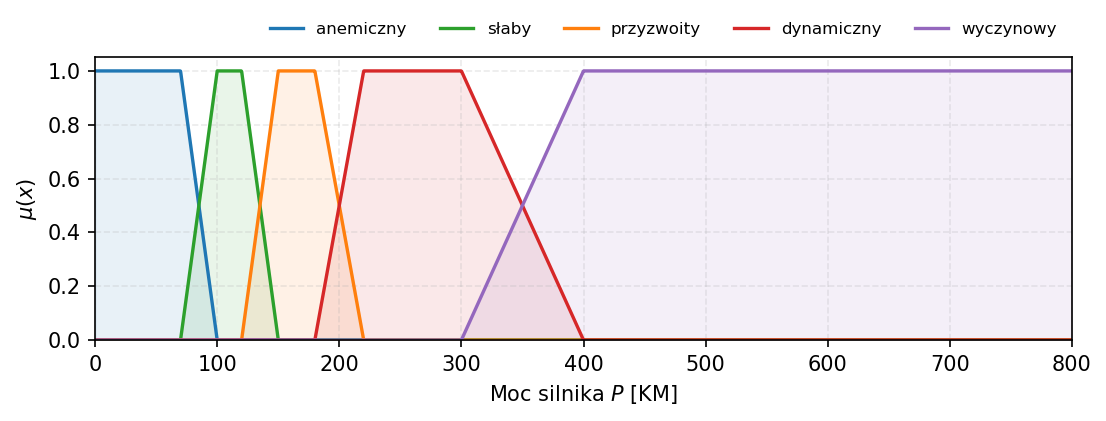
\includegraphics[width=0.9\textwidth]{mf_engine_hp.png}
\caption{Funkcje przynależności pięciu etykiet zmiennej lingwistycznej
,,moc silnika'' $P \in [0, 800]$~KM. Zauważalne liniowe przejścia
w~punktach 50\,\%-stopnia przynależności (np. dla $P=100$~KM:
$\mu_{\text{anemiczny}}(P)=\mu_{\text{słaby}}(P)=0{,}5$) ilustrują rozmyte
pokrycie zupełne wymagane konstrukcją trapezów.}
\label{fig:mf-engine-hp}
\end{figure}

\subsubsection{Średnica zawracania (\texttt{turning\_circle\_m}), $X = [5, 20]$ m}
\begin{table}[H]
\centering
\caption{Parametry trapezowych funkcji przynależności dla zmiennej
,,średnica zawracania''.}
\label{tab:mf-turn}
\begin{tabular}{l r r r r}
\toprule
Etykieta & $a$ & $b$ & $c$ & $d$ \\
\midrule
zwinny       &  5{,}0 &  5{,}0 &  9{,}5 & 10{,}0 \\
zwrotny      &  9{,}5 & 10{,}0 & 10{,}5 & 11{,}0 \\
przeciętny   & 10{,}5 & 11{,}0 & 11{,}3 & 11{,}7 \\
nieporęczny  & 11{,}3 & 11{,}7 & 12{,}5 & 13{,}5 \\
ociężały     & 12{,}5 & 13{,}5 & 20{,}0 & 20{,}0 \\
\bottomrule
\end{tabular}
\end{table}
\begin{figure}[H]
\centering
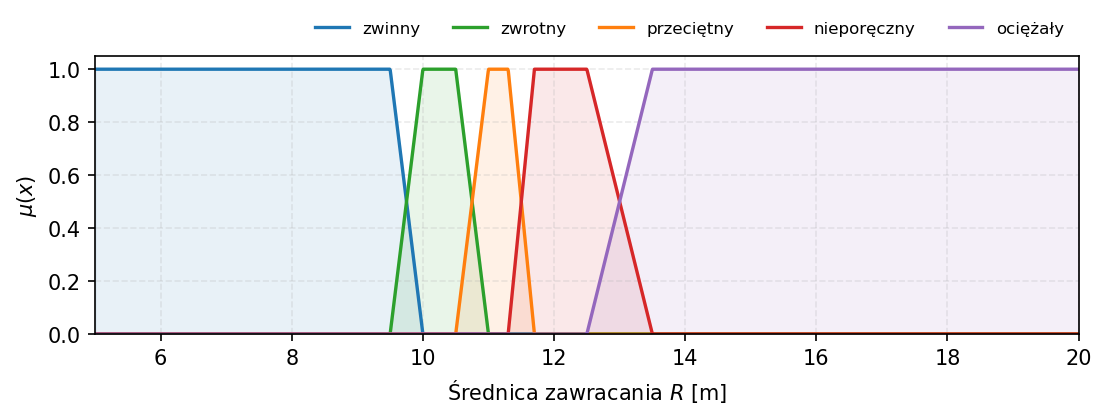
\includegraphics[width=0.9\textwidth]{mf_turning_circle_m.png}
\caption{Funkcje przynależności pięciu etykiet zmiennej lingwistycznej
,,średnica zawracania'' $R \in [5, 20]$~m.}
\label{fig:mf-turn}
\end{figure}

\subsubsection{Spalanie mieszane (\texttt{mixed\_fuel\_consumption\_per\_100\_km\_l}), $X = [0, 25]$ l/100~km}
\begin{table}[H]
\centering
\caption{Parametry trapezowych funkcji przynależności dla zmiennej
,,spalanie mieszane''.}
\label{tab:mf-fuel}
\begin{tabular}{l r r r r}
\toprule
Etykieta & $a$ & $b$ & $c$ & $d$ \\
\midrule
oszczędny    &  0 &  0 &  4 &  5 \\
ekonomiczny  &  4 &  5 &  6 &  7 \\
umiarkowany  &  6 &  7 &  8 & 10 \\
paliwożerny  &  8 & 10 & 12 & 15 \\
rozrzutny    & 12 & 15 & 25 & 25 \\
\bottomrule
\end{tabular}
\end{table}
\begin{figure}[H]
\centering
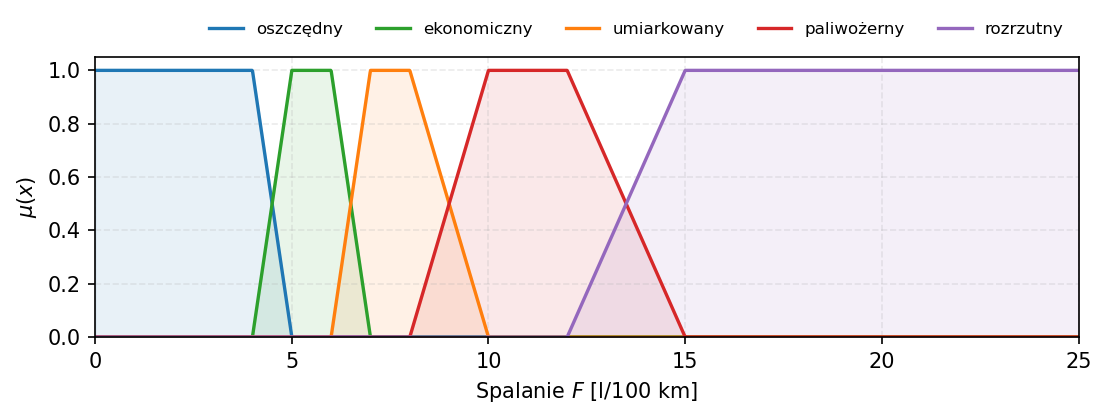
\includegraphics[width=0.9\textwidth]{mf_mixed_fuel_consumption_per_100_km_l.png}
\caption{Funkcje przynależności pięciu etykiet zmiennej lingwistycznej
,,spalanie mieszane'' $F \in [0, 25]$~l/100~km.}
\label{fig:mf-fuel}
\end{figure}

\subsubsection{Pojemność zbiornika paliwa (\texttt{fuel\_tank\_capacity\_l}), $X = [10, 160]$ l}
\begin{table}[H]
\centering
\caption{Parametry trapezowych funkcji przynależności dla zmiennej
,,pojemność zbiornika paliwa''.}
\label{tab:mf-tank}
\begin{tabular}{l r r r r}
\toprule
Etykieta & $a$ & $b$ & $c$ & $d$ \\
\midrule
mały         & 10 & 10 & 40 & 45 \\
niewielki    & 40 & 45 & 50 & 55 \\
standardowy  & 50 & 55 & 65 & 70 \\
pojemny      & 65 & 70 & 80 & 90 \\
ogromny      & 80 & 90 & 160 & 160 \\
\bottomrule
\end{tabular}
\end{table}
\begin{figure}[H]
\centering
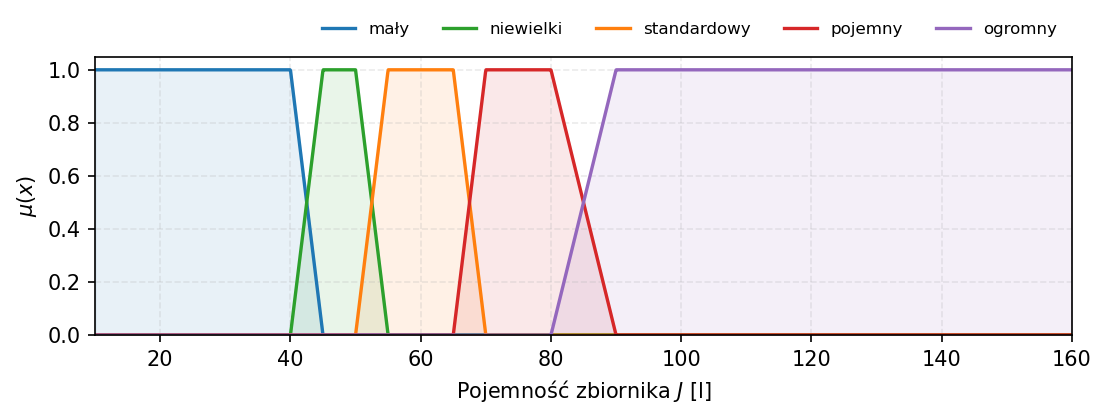
\includegraphics[width=0.9\textwidth]{mf_fuel_tank_capacity_l.png}
\caption{Funkcje przynależności pięciu etykiet zmiennej lingwistycznej
,,pojemność zbiornika paliwa'' $J \in [10, 160]$~l.}
\label{fig:mf-tank}
\end{figure}

\subsubsection{Czas przyspieszenia 0--100 km/h (\texttt{acceleration\_0\_100\_km/h\_s}), $X = [2, 25]$ s}
\begin{table}[H]
\centering
\caption{Parametry trapezowych funkcji przynależności dla zmiennej
,,czas przyspieszenia 0--100~km/h''. Etykiety opisują samochód
poprzez jego dynamikę: niska wartość czasu odpowiada autu
,,rakietowemu'', wysoka -- ,,ślamazarnemu''.}
\label{tab:mf-accel}
\begin{tabular}{l r r r r}
\toprule
Etykieta & $a$ & $b$ & $c$ & $d$ \\
\midrule
rakietowy   &  2 &  2 &  5 &  6 \\
szybki      &  5 &  6 &  8 &  9 \\
przeciętny  &  8 &  9 & 11 & 13 \\
ospały      & 11 & 13 & 15 & 17 \\
ślamazarny  & 15 & 17 & 25 & 25 \\
\bottomrule
\end{tabular}
\end{table}
\begin{figure}[H]
\centering
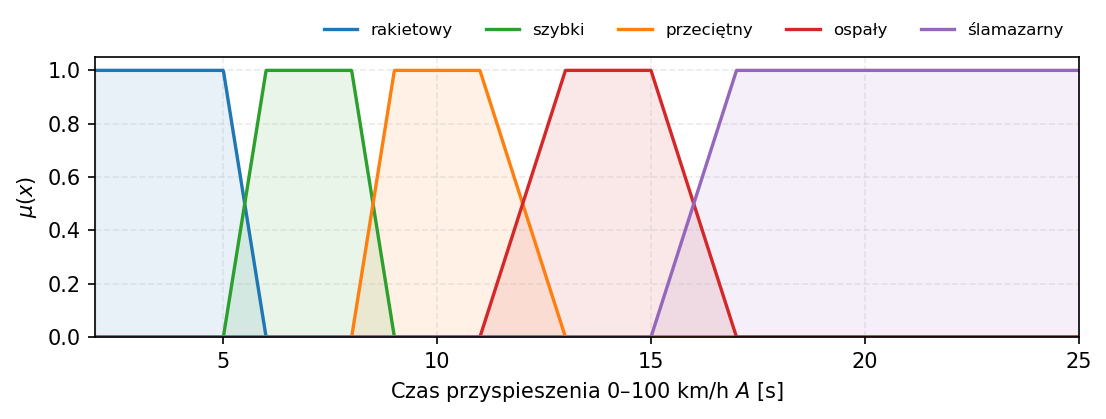
\includegraphics[width=0.9\textwidth]{mf_acceleration_0_100_s.png}
\caption{Funkcje przynależności pięciu etykiet zmiennej lingwistycznej
,,czas przyspieszenia 0--100~km/h'' $A \in [2, 25]$~s. Niskie wartości
$A$ ($<$5~s) odpowiadają samochodom szybkim, wysokie ($>$15~s) --
samochodom wolnym.}
\label{fig:mf-accel}
\end{figure}

\subsubsection{Prędkość maksymalna (\texttt{max\_speed\_km\_per\_h}), $X = [80, 360]$ km/h}
\begin{table}[H]
\centering
\caption{Parametry trapezowych funkcji przynależności dla zmiennej
,,prędkość maksymalna''.}
\label{tab:mf-vmax}
\begin{tabular}{l r r r r}
\toprule
Etykieta & $a$ & $b$ & $c$ & $d$ \\
\midrule
powolny       &  80 &  80 & 150 & 165 \\
miejski       & 150 & 165 & 180 & 195 \\
autostradowy  & 180 & 195 & 210 & 230 \\
wyścigowy     & 210 & 230 & 250 & 280 \\
błyskawiczny  & 250 & 280 & 360 & 360 \\
\bottomrule
\end{tabular}
\end{table}
\begin{figure}[H]
\centering
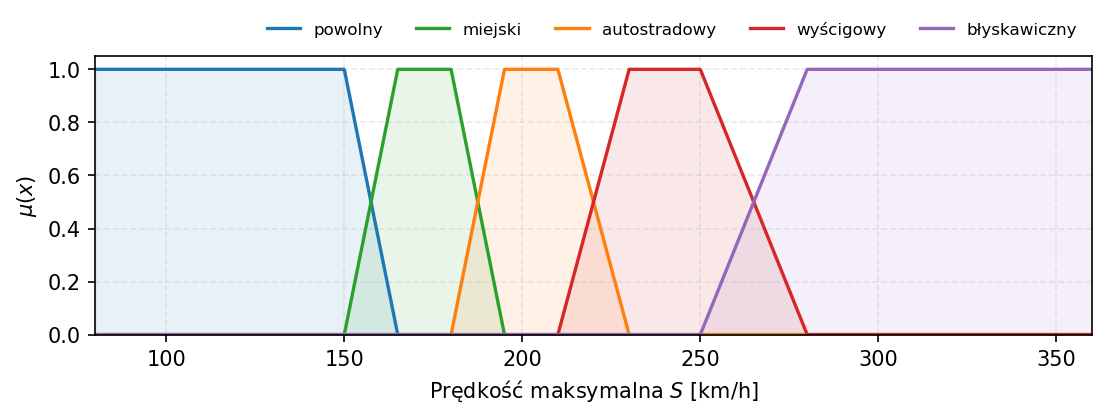
\includegraphics[width=0.9\textwidth]{mf_max_speed_km_per_h.png}
\caption{Funkcje przynależności pięciu etykiet zmiennej lingwistycznej
,,prędkość maksymalna'' $S \in [80, 360]$~km/h.}
\label{fig:mf-vmax}
\end{figure}

% --------------------------------------------------------------
\subsection{Kwantyfikatory lingwistyczne (liczności obiektów)}
\label{sec:quant}

\textbf{Kwantyfikatory lingwistyczne} to słowa, które w zdaniu
,,$Q$ obiektów ze zbioru ma własność $S$'' stoją w miejscu $Q$ --
np. ,,większość'', ,,około połowy'', ,,prawie wszystkie''. Każdy
kwantyfikator opisujemy zbiorem rozmytym z trapezową funkcją
przynależności, dokładnie tak samo jak zmienne lingwistyczne
(\S\ref{sec:zmienne}), tylko że na innej dziedzinie. Rozróżniamy
dwa rodzaje kwantyfikatorów:
\begin{itemize}
    \item \textbf{względne (proporcjonalne)} -- argumentem jest
    \emph{udział} obiektów spełniających warunek, $r \in [0,1]$
    (np. ,,około połowy'' = $r \approx 0{,}5$);
    \item \textbf{bezwzględne (absolutne)} -- argumentem jest
    \emph{liczba} obiektów spełniających warunek, $r \in \mathbb{N}$
    (np. ,,kilka tysięcy'' = $r \approx$ kilka tysięcy rekordów).
\end{itemize}

\subsubsection{Kwantyfikatory względne}

Przestrzeń rozważań $X_Q = [0, 1]$. Pięć etykiet pokrywa cały odcinek
$[0,1]$ z~przejściami w okolicach typowych progów intuicji
($\sim$0,1 -- ,,prawie żaden'', $\sim$0,5 -- ,,około połowy'',
$\sim$0,9 -- ,,prawie wszystkie'').

\begin{table}[H]
\centering
\caption{Parametry trapezowych funkcji przynależności pięciu
kwantyfikatorów względnych. Argumentem jest proporcja
$r \in [0,1]$ obiektów spełniających warunek.}
\label{tab:q-relative}
\begin{tabular}{l r r r r}
\toprule
Etykieta & $a$ & $b$ & $c$ & $d$ \\
\midrule
prawie żaden     & 0{,}00 & 0{,}00 & 0{,}05 & 0{,}20 \\
mniejszość       & 0{,}05 & 0{,}20 & 0{,}30 & 0{,}40 \\
około połowy     & 0{,}30 & 0{,}40 & 0{,}60 & 0{,}70 \\
większość        & 0{,}60 & 0{,}70 & 0{,}85 & 0{,}95 \\
prawie wszystkie & 0{,}85 & 0{,}95 & 1{,}00 & 1{,}00 \\
\bottomrule
\end{tabular}
\end{table}
\begin{figure}[H]
\centering
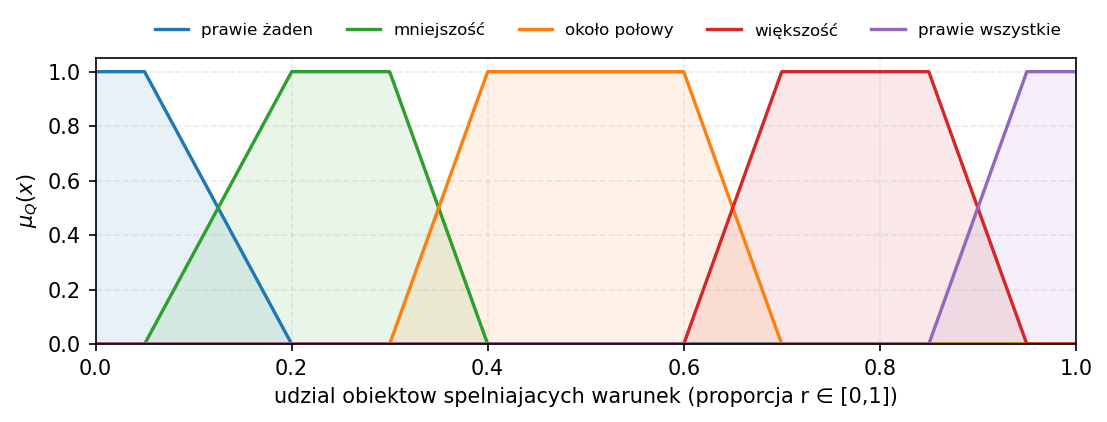
\includegraphics[width=0.9\textwidth]{quantifiers_relative.png}
\caption{Funkcje przynależności pięciu kwantyfikatorów względnych
zdefiniowanych na przestrzeni $X_Q = [0, 1]$. Argumentem
jest proporcja obiektów spełniających warunek (np. $r=0{,}5$:
$\mu_{\text{około połowy}}=1$).}
\label{fig:quant-rel}
\end{figure}

\subsubsection{Kwantyfikatory bezwzględne}

Przestrzeń rozważań $X_Q^{\text{abs}} = [0, 25\,000]$ -- górna granica
wzięta nieco powyżej liczności podzbioru roboczego ($23\,441$
rekordów), aby etykieta ,,dużo'' była aktywna dla niemal całej
populacji bazy, gdy podsumowanie obejmuje praktycznie wszystkie
rekordy. Przyjęto cztery etykiety zamiast pięciu, ponieważ na osi
liczności (w~przeciwieństwie do osi proporcji) różnice rzędu wielkości
są bardziej istotne niż różnice o~stałym kroku, a~granice odpowiadają
intuicji ,,bardzo mało / kilka tysięcy / kilkanaście tysięcy / dużo''.

\begin{table}[H]
\centering
\caption{Parametry trapezowych funkcji przynależności czterech
kwantyfikatorów bezwzględnych. Argumentem jest liczba (rekordów) obiektów
spełniających warunek.}
\label{tab:q-absolute}
\begin{tabular}{l r r r r}
\toprule
Etykieta & $a$ & $b$ & $c$ & $d$ \\
\midrule
bardzo mało           &      0 &      0 &  1\,000 &  3\,000 \\
kilka tysięcy         &  1\,000 &  3\,000 &  6\,000 &  8\,000 \\
kilkanaście tysięcy   &  6\,000 &  8\,000 & 14\,000 & 16\,000 \\
dużo                  & 14\,000 & 16\,000 & 25\,000 & 25\,000 \\
\bottomrule
\end{tabular}
\end{table}
\begin{figure}[H]
\centering
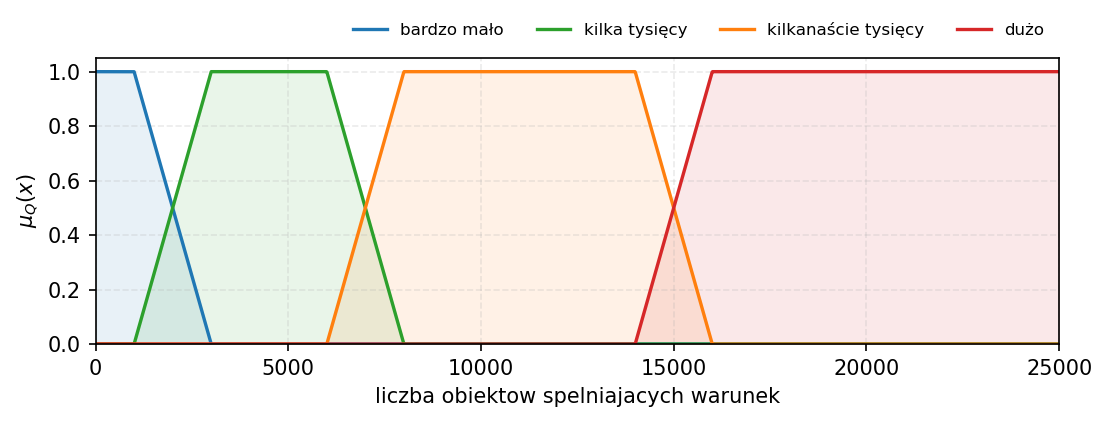
\includegraphics[width=0.9\textwidth]{quantifiers_absolute.png}
\caption{Funkcje przynależności czterech kwantyfikatorów bezwzględnych
zdefiniowanych na przestrzeni $X_Q^{\text{abs}} = [0, 25\,000]$.
Argumentem jest liczba obiektów spełniających warunek.}
\label{fig:quant-abs}
\end{figure}


% =====================================================================
\section{Narzędzia obliczeniowe: wybór/implementacja. Diagram UML klas do obliczeń rozmytych i generowania podsumowań}
\noindent {\bf Sekcja uzupełniona jako efekt zadania Tydzień 10 wg Harmonogramu Zajęć na WIKAMP KSR.}

Diagram UML i zwięzły opis pakietu obliczeń rozmytych: źródło pakietu
(zewnętrzny/własny/hybrydowy), przypis do literatury/źródeł. Krótka charakterystyka
najważniejszych klas i podstawowych dla zadania ich metod. \\

Wersja JRE i inne wymogi niezbędne do uruchomienia aplikacji przez użytkownika na własnym komputerze.

% =====================================================================
\section{Jednopodmiotowe podsumowania lingwistyczne. Miary jakości, podsumowanie optymalne}
Wyniki kolejnych eksperymentów wg punktów 2.-4. opisu projektu 2.  Listy podsumowań
jednopodmiotowych i tabele/rankingi podsumowań dla danych atrybutów obowiązkowe i dokładnie opisane w ,,captions'' (tytułach), konieczny opis kolumn i wierszy tabel. Dla każdego podsumowania podane miary jakości oraz miara jakości podsumowania
optymalnego. {\bf Wzorów podsumowań ani miar nie należy przepisywać ani cytować, wystarczy podać literaturę, ale
należy skomentować co oznaczają i jaką informacje niosą wybrane miary w wybranych
przypadkach.}\\
\noindent {\bf Sekcja uzupełniona jako efekt zadania Tydzień 11 wg Harmonogramu Zajęć na WIKAMP KSR.}

% =====================================================================
\section{Wielopodmiotowe podsumowania lingwistyczne i~ich miary jakości}
Wyniki kolejnych eksperymentów wg punktów 2.-4. opisu projektu 2. Uzasadnienie i
metoda podziału zbioru danych na rozłączne podmioty. Listy podsumowań
wielopodmiotowych i tabele/rankingi podsumowań dla danych atrybutów obowiązkowe i
dokładnie opisane w ,,captions'' (tytułach), konieczny opis kolumn i wierszy tabel.
{\bf Wzorów podsumowań ani miar nie należy przepisywać ani cytować, wystarczy podać literaturę, ale
należy skomentować co oznaczają i jaką informacje niosą wybrane miary w wybranych
przypadkach.} Konieczne uwzględnienie wszystkich 4-ch form podsumowań wielopodmiotowych.
\\

** Możliwe sformułowanie zagadnienia wielopodmiotowego podsumowania optymalnego **.\\
\indent {** Ewentualne wyniki realizacji punktu ,,na ocenę 5.0'' wg opisu Projektu 2. i ich porównanie do wyników z
części obowiązkowej **.}\\

\noindent {\bf Sekcja uzupełniona jako efekt zadania Tydzień 12 wg Harmonogramu Zajęć
na WIKAMP KSR.}


% =====================================================================
\section{Dyskusja, wnioski}
We wnioskach z badania skomentować wyłącznie wpływ wybranych parametrów (zbiorów rozmytych, zmiennych lingwistycznych, miar podobieństwa, itp.) na jakość procesu klasyfikacji. Innymi słowy – wnioski to to, co wynika z przeprowadzonych obliczeń, a nie to co wiadomo z literatury. \\
Komentować należy wyłącznie zbiór danych i zanczenie otrzymanych podsumowań. Metody nie komentujemy. \\
Dokładne interpretacje uzyskanych wyników w zależności od parametrów
opisanych w punktach 3.-4 opisu Projektu 2.
Omówić i wyjaśnić napotkane problemy (jeśli były). Każdy wniosek/problem powinien mieć poparcie
w przeprowadzonych eksperymentach (odwołania do konkretnych wyników: podsumowań i miar
jakości). Ocena które podsumowania i dlaczego niosą najistotniejsze informacje
i które ich miary jakości mają małe albo duże znaczenie dla wiarygodności i jakości otrzymanych
agregacji/podsumowań.  \\
\underline{Dla końcowej oceny jest to najważniejsza sekcja} sprawozdania, gdyż prezentuje poziom
zrozumienia rozwiązywanego problemu.\\

** Możliwości kontynuacji prac w obszarze logiki rozmytej i wnioskowania rozmytego, zwłaszcza w kontekście pracy inżynierskiej,
magisterskiej, naukowej, itp. **\\

\noindent {\bf Sekcja uzupełniona jako efekt zadań Tydzień 11 i Tydzień 12 wg
Harmonogramu Zajęć na WIKAMP KSR.}


% =====================================================================
\section{Braki w realizacji projektu 2.}
Wymienić wg opisu Projektu 2. wszystkie niezrealizowane obowiązkowe elementy projektu, ewentualnie
podać merytoryczne (ale nie czasowe) przyczyny tych braków.


% =====================================================================
\begin{thebibliography}{99}

\bibitem{niewiadomski19} A. Niewiadomski,
\textit{Zbiory rozmyte typu 2. Zastosowania w reprezentowaniu informacji},
Seria ,,Problemy współczesnej informatyki'' pod redakcją L. Rutkowskiego,
Akademicka Oficyna Wydawnicza EXIT, Warszawa, 2019.

\bibitem{zadrozny06} S. Zadrożny,
\textit{Zapytania nieprecyzyjne i lingwistyczne podsumowania baz danych},
EXIT, Warszawa, 2006.

\bibitem{niewiadomski08} A. Niewiadomski,
\textit{Methods for the Linguistic Summarization of Data: Applications of
Fuzzy Sets and Their Extensions}, Akademicka Oficyna Wydawnicza EXIT,
Warszawa, 2008.

\bibitem{zadeh75} L.~A. Zadeh,
,,The concept of a linguistic variable and its application to approximate
reasoning'', \textit{Information Sciences}, vol. 8, nr 3, ss. 199--249, 1975.

\bibitem{zadeh83} L.~A. Zadeh,
,,A computational approach to fuzzy quantifiers in natural languages'',
\textit{Computers \& Mathematics with Applications}, vol. 9, nr 1,
ss. 149--184, 1983.

\bibitem{yager82} R.~R. Yager,
,,A new approach to the summarization of data'',
\textit{Information Sciences}, vol. 28, nr 1, ss. 69--86, 1982.

\bibitem{kacprzyk-yager01} J. Kacprzyk, R.~R. Yager,
,,Linguistic summaries of data using fuzzy logic'',
\textit{International Journal of General Systems}, vol. 30, nr 2,
ss. 133--154, 2001.

\bibitem{kaggle-cars} J. Islam,
\textit{Car Specification Dataset 1945--2020}, Kaggle, 2020.\\
\url{https://www.kaggle.com/datasets/jahaidulislam/car-specification-dataset-1945-2020}

\end{thebibliography}

Literatura zawiera wyłącznie źródła recenzowane i/lub o potwierdzonej wiarygodności,
możliwe do weryfikacji i cytowane w sprawozdaniu.
\end{document}
